% ==============================================================================
% CHAPTER 7: REPRESENTATIVE SYSTEM PLATFORMS AND STANDARD BENCHMARK DATASETS
% ==============================================================================
\section{Representative System Platforms and Standard Benchmark Datasets}
\label{sec:platform_benchmarks}

The preceding chapters examined how multi-agent collaborative QA systems are
organised, implemented, and selected for particular application settings. To
make these design choices reproducible in practice, researchers also need two
complementary types of resources: platforms for prototyping and deployment,
and benchmarks for evaluating systems under comparable conditions. This
section maps these resources without treating platform adoption or benchmark
scores as evidence of universal system superiority. Platforms determine which
coordination and knowledge-processing capabilities can be instantiated,
whereas benchmarks determine which aspects of QA behaviour are measured.

\subsection{A Layered View of System Platforms and Selection Boundaries}
\label{sec:platform_layers}

The current development ecosystem can be viewed as three functional layers.
At the foundation layer, general-purpose development frameworks, such as
LangChain and LlamaIndex, provide model interfaces, retrieval components, and
tool integrations. They are useful infrastructure, but they do not by
themselves prescribe a multi-agent QA organisation. At the orchestration
layer, general multi-agent frameworks, including AutoGen, CrewAI, and MetaGPT,
provide abstractions for role definition, message exchange, and workflow
control. These frameworks are broadly reusable, although developers must
still construct task-specific document-processing and QA pipelines. At the
application-resource layer, systems concentrate capabilities around a more
specific information-seeking or knowledge-service workflow.

Figure~\ref{fig:platform_resource_map} provides an overview of how these
platform layers connect a multi-agent QA system to representative resources
and complementary evaluation settings. It is a conceptual resource map rather
than a performance ranking or a causal model of system quality.

\begin{figure*}[t]
  \centering
  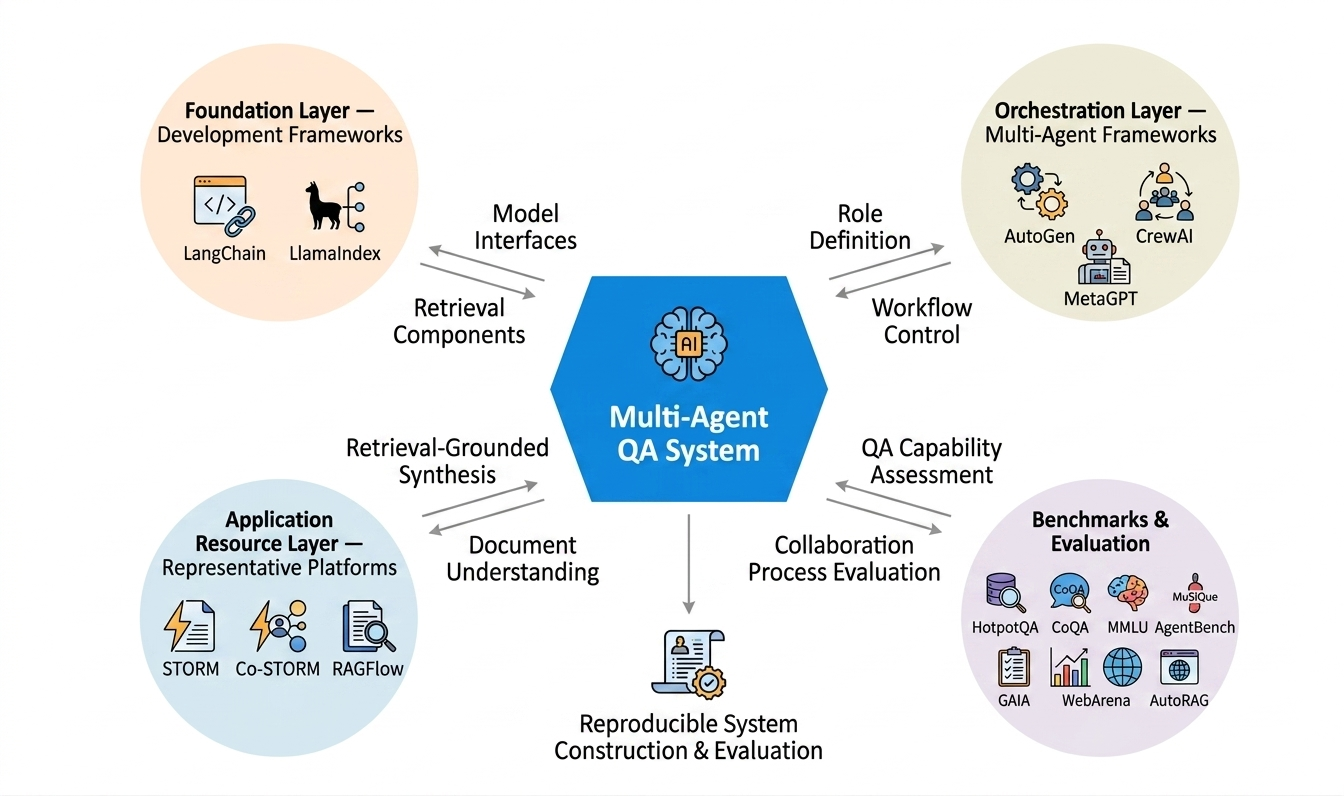
\includegraphics[width=0.94\textwidth]{classify.jpg}
  \caption{Layered resource ecosystem for reproducible construction and
  evaluation of multi-agent collaborative QA systems.}
  \label{fig:platform_resource_map}
\end{figure*}

This review focuses on the last layer through three complementary resources:
STORM, Co-STORM, and RAGFlow. STORM and Co-STORM exemplify multi-perspective,
retrieval-grounded information seeking and synthesis; RAGFlow is an
open-source RAG engine oriented towards deep document understanding and
knowledge-base workflows. They should therefore be read as representative
resource configurations rather than as a controlled ranking of systems. The
choice among them depends on whether the intended QA task emphasises
open-ended research and synthesis, user-steered exploration, or document-rich
enterprise knowledge access.

\subsection{Representative Resource Configurations}
\label{sec:representative_platforms}

STORM (Synthesis of Topic Outlines through Retrieval and Multi-perspective
Question Asking) structures long-form, source-grounded writing around
perspective discovery, simulated question--answer conversations, and
outline-guided synthesis \citep{shao2024storm}. Its design is particularly
relevant when a system must expand an initially broad topic into a structured
research report. Co-STORM extends this setting by allowing users to observe
and steer a discourse among language-model agents; a dynamic mind map records
the information uncovered during the interaction \citep{shao2024costorm}.
This makes it a useful reference point for human-in-the-loop (HITL)
information exploration, in which the user can redirect the collaboration
rather than only accept its final output.

Figure~\ref{fig:costorm_mindmap} illustrates the role of a mind map as an
interaction record in Co-STORM. Such a representation can help make the
evolving discourse visible to a user, but its presence alone does not provide
a complete audit trail. High-stakes deployments still require explicit
provenance, approval, and responsibility mechanisms, as discussed in
Section~8.

\begin{figure*}[t]
  \centering
  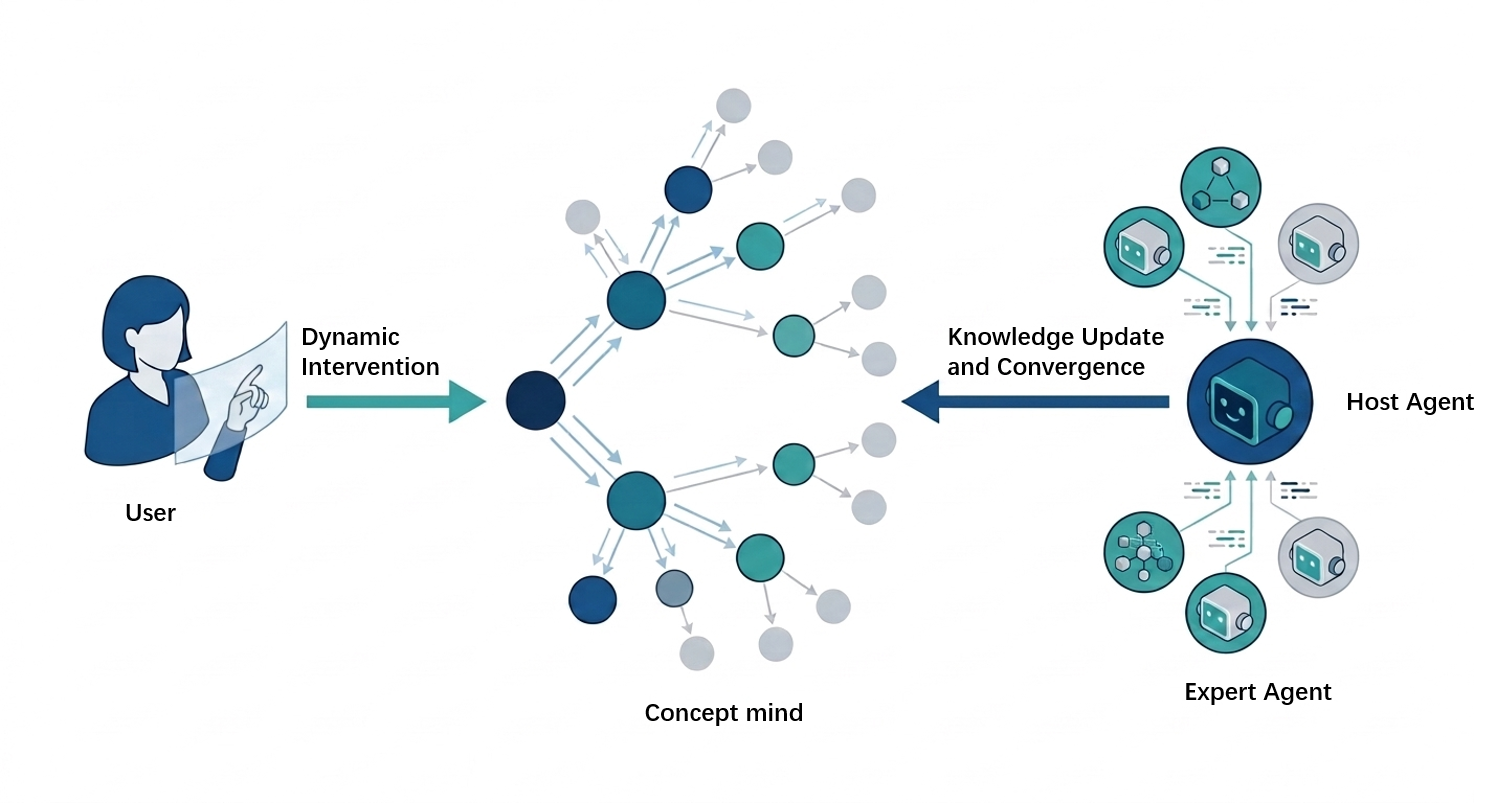
\includegraphics[width=0.92\textwidth]{findmap.png}
  \caption{Mind-map-mediated human--agent interaction in Co-STORM, adapted
  from \citet{shao2024costorm}.}
  \label{fig:costorm_mindmap}
\end{figure*}

RAGFlow addresses a different but complementary engineering requirement. As
an open-source RAG engine, it places deep document understanding at the centre
of knowledge ingestion and retrieval workflows \citep{ragflow2024}. Its
document-processing orientation is relevant when QA quality depends on
extracting usable evidence from heterogeneous enterprise or technical
documents. In this context, deep document understanding (DDU) denotes
document parsing that aims to preserve structures such as layouts, tables, and
other content required for subsequent retrieval and answer generation.

Table~\ref{tab:platform_capability_matrix} compares the distinct
configurations represented by these systems. The comparison is descriptive:
it identifies the resource and interaction assumptions that a practitioner
would need to inspect when translating an architecture choice into a concrete
implementation.

\begin{table*}[t]
  \centering
  \caption{Representative platform configurations for multi-agent collaborative QA.}
  \label{tab:platform_capability_matrix}
  \small
  \begin{tabularx}{\textwidth}{p{3.0cm} X X X}
    \toprule
    \textbf{Capability dimension} & \textbf{STORM} & \textbf{Co-STORM} & \textbf{RAGFlow} \\
    \midrule
    Primary resource orientation &
    Retrieval-grounded long-form knowledge synthesis &
    User-participatory information exploration and report synthesis &
    Document-centred RAG and knowledge-base workflows \\
    Collaboration or workflow mechanism &
    Multi-perspective questioning, simulated conversations, and outline-guided writing &
    Multi-agent discourse with a moderator and a dynamic mind map for interaction tracking &
    Document ingestion, retrieval, and configurable workflow components \\
    Human-control point &
    Primarily topic and report specification before synthesis &
    Users may observe and steer the ongoing discourse &
    Workflow and knowledge-base configuration for deployment contexts \\
    Best-matched QA setting &
    Broad research or explanatory questions requiring structured synthesis &
    Exploratory questions for which user intent may evolve during interaction &
    QA over heterogeneous, document-rich organisational knowledge \\
    Selection boundary &
    Does not substitute for robust local-document parsing or high-stakes review controls &
    Human participation requires explicit intervention and accountability policies &
    Document understanding alone does not establish multi-agent reasoning quality \\
    \bottomrule
  \end{tabularx}
\end{table*}

\subsection{Standard Benchmarks for QA and Agent Interaction}
\label{sec:benchmark_datasets}

Benchmark resources should be matched to the system property being assessed.
Conventional QA datasets are useful for testing retrieval, multi-hop
reasoning, conversational context handling, and broad knowledge coverage.
Agent-oriented environments additionally test planning, tool use, and
long-horizon interaction. Neither class alone is sufficient for assessing a
multi-agent QA system: a system can answer a static question correctly while
using an inefficient collaboration process, or it can execute tools
successfully without providing reliable evidence for an answer.

HotpotQA provides Wikipedia-based multi-hop questions with sentence-level
supporting facts, making it appropriate for evaluating evidence-grounded
retrieval and reasoning \citep{yang2018hotpotqa}. CoQA evaluates
context-dependent conversational QA through connected question--answer
turns \citep{reddy2019coqa}. MMLU tests broad multi-task knowledge and
reasoning across academic subjects \citep{hendrycks2021mmlu}, whereas MuSiQue
constructs multi-hop questions from single-hop components to probe connected
reasoning \citep{trivedi2022musique}. These resources assess answer-focused
capabilities, but they provide limited direct evidence about an agent team's
planning or tool-use process.

AgentBench, GAIA, and WebArena extend evaluation towards interactive settings.
AgentBench evaluates LLM agents across eight environments involving reasoning
and decision-making \citep{liu2024agentbench}; GAIA combines reasoning with
multi-modal information and tool-use requirements for general AI assistants
\citep{mialon2024gaia}; and WebArena supplies reproducible web environments
for long-horizon tasks across common online domains \citep{zhou2024webarena}.
Together, these benchmarks enable a more complete resource map, although
their task definitions, interfaces, and success metrics differ and should not
be merged into a single aggregate score.

\begin{table*}[t]
  \centering
  \caption{Benchmark resources and their primary evaluation role in multi-agent collaborative QA.}
  \label{tab:benchmark_resources}
  \small
  \begin{tabularx}{\textwidth}{p{2.3cm} p{2.6cm} X X}
    \toprule
    \textbf{Resource} & \textbf{Evaluation setting} & \textbf{Primary capability assessed} & \textbf{Interpretation for multi-agent QA} \\
    \midrule
    HotpotQA & Multi-hop QA with supporting facts & Cross-document retrieval, evidence use, and multi-hop reasoning & Tests whether collaboration improves evidence-grounded answer construction \\
    CoQA & Conversational QA & Context retention, coreference handling, and answer consistency across turns & Tests memory and dialogue coordination under connected QA turns \\
    MMLU & Multi-subject multiple-choice tasks & Broad knowledge and subject-specific reasoning & Provides a knowledge-reasoning baseline, not a direct measure of collaboration quality \\
    MuSiQue & Compositional multi-hop QA & Connected reasoning across linked subquestions & Tests decomposition and evidence chaining relevant to specialised agent roles \\
    AgentBench & Interactive agent environments & Reasoning, decision-making, and environment interaction & Tests tool- and environment-facing agent behaviour beyond static answers \\
    GAIA & General-assistant tasks & Reasoning, information access, and tool use & Tests integrated task completion requiring heterogeneous capabilities \\
    WebArena & Reproducible web environments & Long-horizon web interaction and functional task completion & Tests planning and action execution in realistic online workflows \\
    \bottomrule
  \end{tabularx}
\end{table*}

\subsection{Automated Evaluation and Optimisation Tools}
\label{sec:automated_evaluation_tools}

Static benchmarks can be complemented by tools that automate the comparison
of retrieval-augmented generation (RAG) configurations. AutoRAG searches for
RAG-module combinations that are suitable for a given dataset and reports
the resulting evaluation outcomes \citep{autorag2024}. For multi-agent QA,
such tooling can be used to evaluate retrieval and generation components
inside a broader collaboration workflow. It should not, however, be taken as
an evaluation of the collaboration policy itself: agent selection,
communication, disagreement resolution, and human intervention require
trace-level measures in addition to final-answer scores.

In summary, platform resources address where and how a multi-agent QA system
can be assembled, whereas datasets and evaluation tools address which
behaviours can be measured during development. Their joint use supports
reproducible system construction, but the appropriate platform and benchmark
remain contingent on the task, evidence source, risk level, and resource
budget. These boundaries motivate the process-aware and risk-adaptive agenda
developed in the following discussion.
